\subsection{Activation} \label{subs:acti}
The activation function is the non-linear output of the neuron. Its purpose is to decide whether the neuron fires or not. In order apply the backpropagation algorithm (see section \ref{sec:train}) to make the network learn, we need to have the activation function to be differentiable \cite{lecun_backpropagation_1989}. Therefore for this reason, we can not use the original perceptron function. Various activations functions have then be proposed with different properties, as illustrated on figure \ref{fig:acti}.
%
\begin{figure}
    \centering
    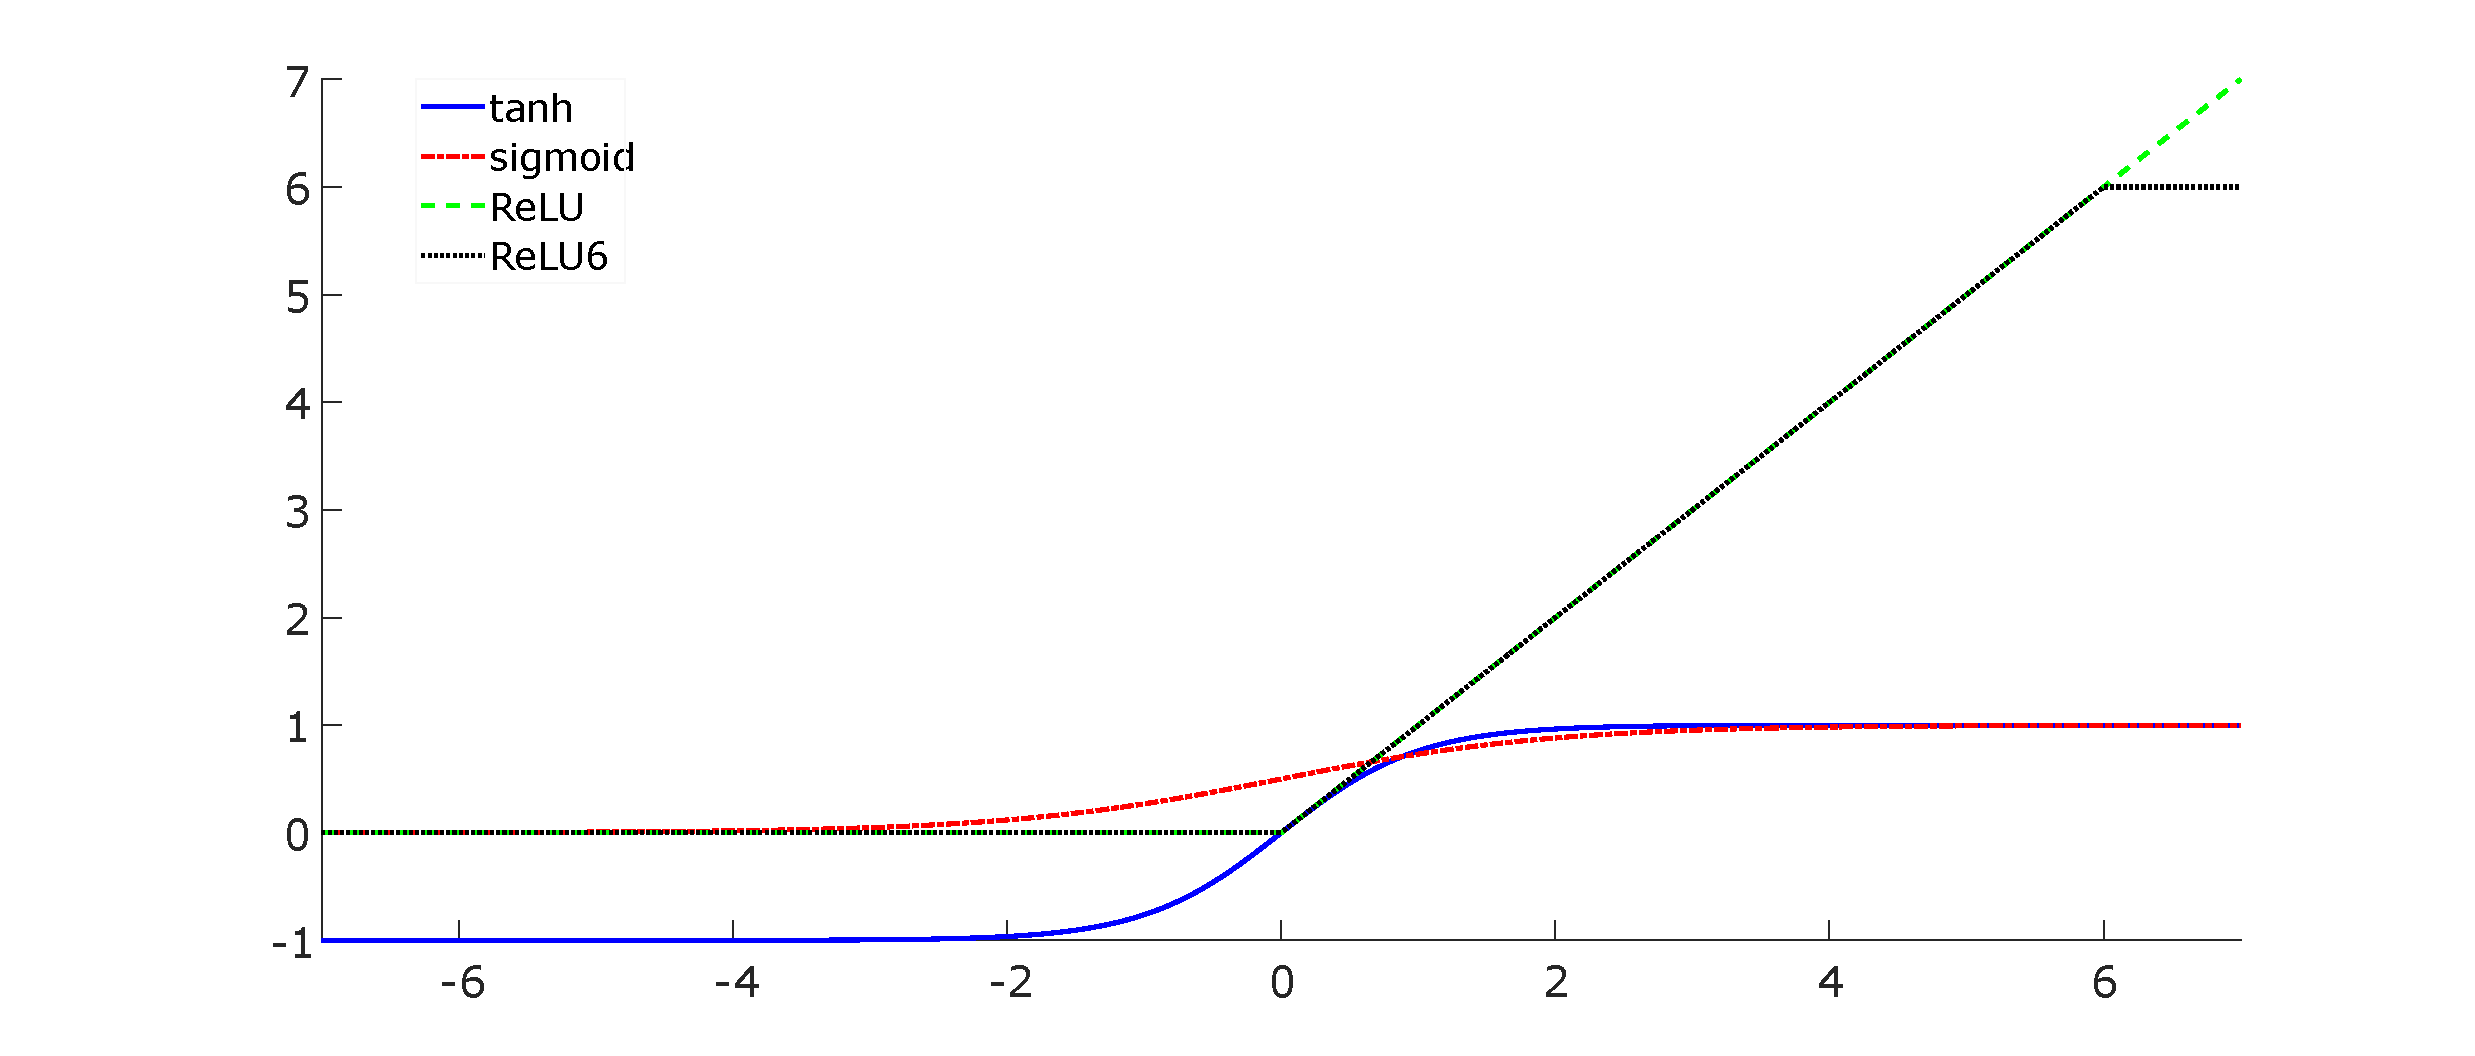
\includegraphics[width=\textwidth]{actifun.pdf}
    \caption{Activation functions}
    \label{fig:acti}
\end{figure}
%
\subsubsection{Sigmoid and Hyperbilolic Tangent (Tanh)}
Sigmoid and tanh functions are both smooth function that can be described by function \eqref{eq:sigmoid} and \eqref{eq:tanh}.
%
\begin{equation}
    h(x) = \frac{1}{1 + e^{-x}}
    \label{eq:sigmoid}
\end{equation}
%
\begin{equation}
    h(x) = \frac{e^{x} - e^{-x}}{e^{x} + e^{-x}}
    \label{eq:tanh}
\end{equation}

The two functions can be seen on figure \ref{fig:acti}. They both 'squeeze' the domain $\mathbb{R}$ into a smaller range, $[0, 1]$ for sigmoid and $[-1, 1]$ for the tanh. However, they also saturate which means their gradient is close to 0. As the bakcpropagation algorithm requires gradient multiplication, gradient far away from the output vanishes and deep models do not learn (\textbf{vanishing gradient problem}) \cite{goodfellow_deep_2016}.
%
\subsubsection{ReLU}
To solve the problem of saturation, the Rectified Linear Unit (ReLU) as been introduced \cite{krizhevsky_imagenet_2012} (see equation \eqref{eq:relu}).
\begin{equation}
    h(x) = max(0, x)
    \label{eq:relu}
\end{equation}

This new activation function allows a faster learning and an efficient gradient propagation (no vanishing or exploding gradient). However, is suffers from the \textbf{dying neurons problems} which decrease the model capacity. The neurons become inactive (outputs only 0) for essentially all inputs and the neuron 'dies'. A solution would be to modify the ReLU: leaky ReLU, ELU, ... \cite{howard_mobilenets_2017} uses ReLU6 (equation \ref{eq:relu6}), that we can see on figure \ref{fig:acti}. It is claimed that it is more robus with low-precision computation.
%
\begin{equation}
    h(x) = max(0, x, 6)
    \label{eq:relu6}
\end{equation}
